\documentclass[11pt]{article}
\usepackage{october}

\begin{document}

\title{Asymmetry and the Geometry of Reason}
\author{Anonymous}
\date{}
\maketitle

\section{Introduction}
\label{intr}

The geometry of reason refers to a view of epistemic utility in which
the underlying topology for credence functions (which may be
subjective probability distributions) on a finite number of events is
a metric space. Since the isomorphism is to a metric space, there is a
distance relation between credence functions which can be used to
formulate axioms relating credences to epistemic utility and to
justify or to criticize contentious positions such as Bayesian
conditionalization, the principle of indifference, other forms of
conditioning, or probabilism itself (see especially works cited below
by James Joyce; Pettigrew and Leitgeb; David Wallace and Hilary
Greaves).

My claim is that given an epistemic utility approach and some
intuitive axioms, the geometry of reason leads itself ad absurdum; and
that there is a viable alternative to the geometry of reason which
avoids the problematic implications: information theory. For
information theory, as opposed to the geometry of reason, the
underlying topology for credence functions is not a metric space (see
figures \ref{fig:contourslp} and \ref{fig:contoursrj} for
illustration).

\begin{figure}[ht]
  \begin{flushright}
    \begin{minipage}[h]{.7\linewidth}
      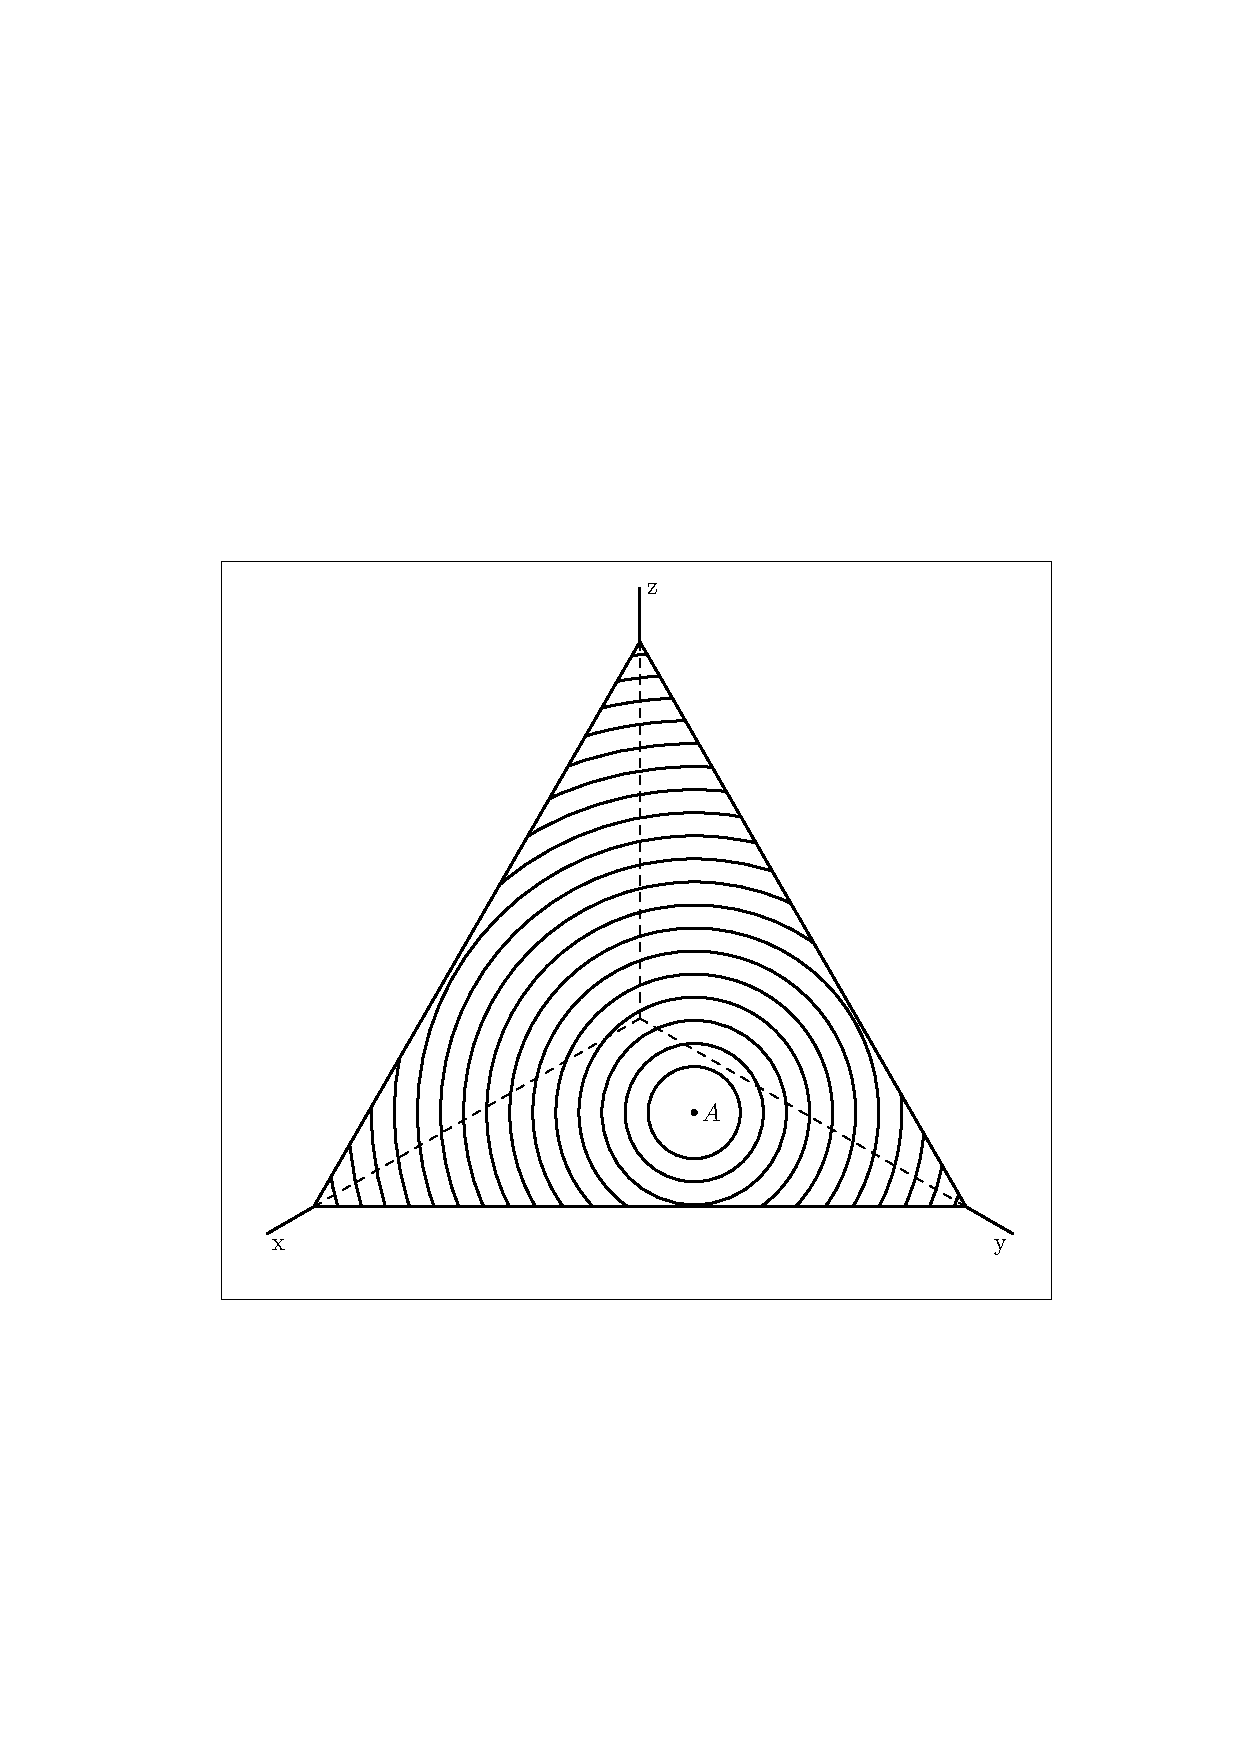
\includegraphics[width=\textwidth]{contourslp.pdf}
      \caption{\footnotesize The simplex $\mathbb{S}^{3}$ in
        three-dimensional space $\mathbb{R}^{3}$ with contour lines
        corresponding to the geometry of reason around point $A$ in
        equation (\ref{eq:e6}). Points on the same contour line are
        equidistant from $A$ with respect to the Euclidean metric.
        Compare the contour lines here to figure
        (\ref{fig:contoursrj}). Note that this diagram and all the
        following diagrams are frontal views of the simplex.}
      \label{fig:contourslp}
    \end{minipage}
  \end{flushright}
\end{figure}

\begin{figure}[ht]
  \begin{flushright}
    \begin{minipage}[h]{.7\linewidth}
      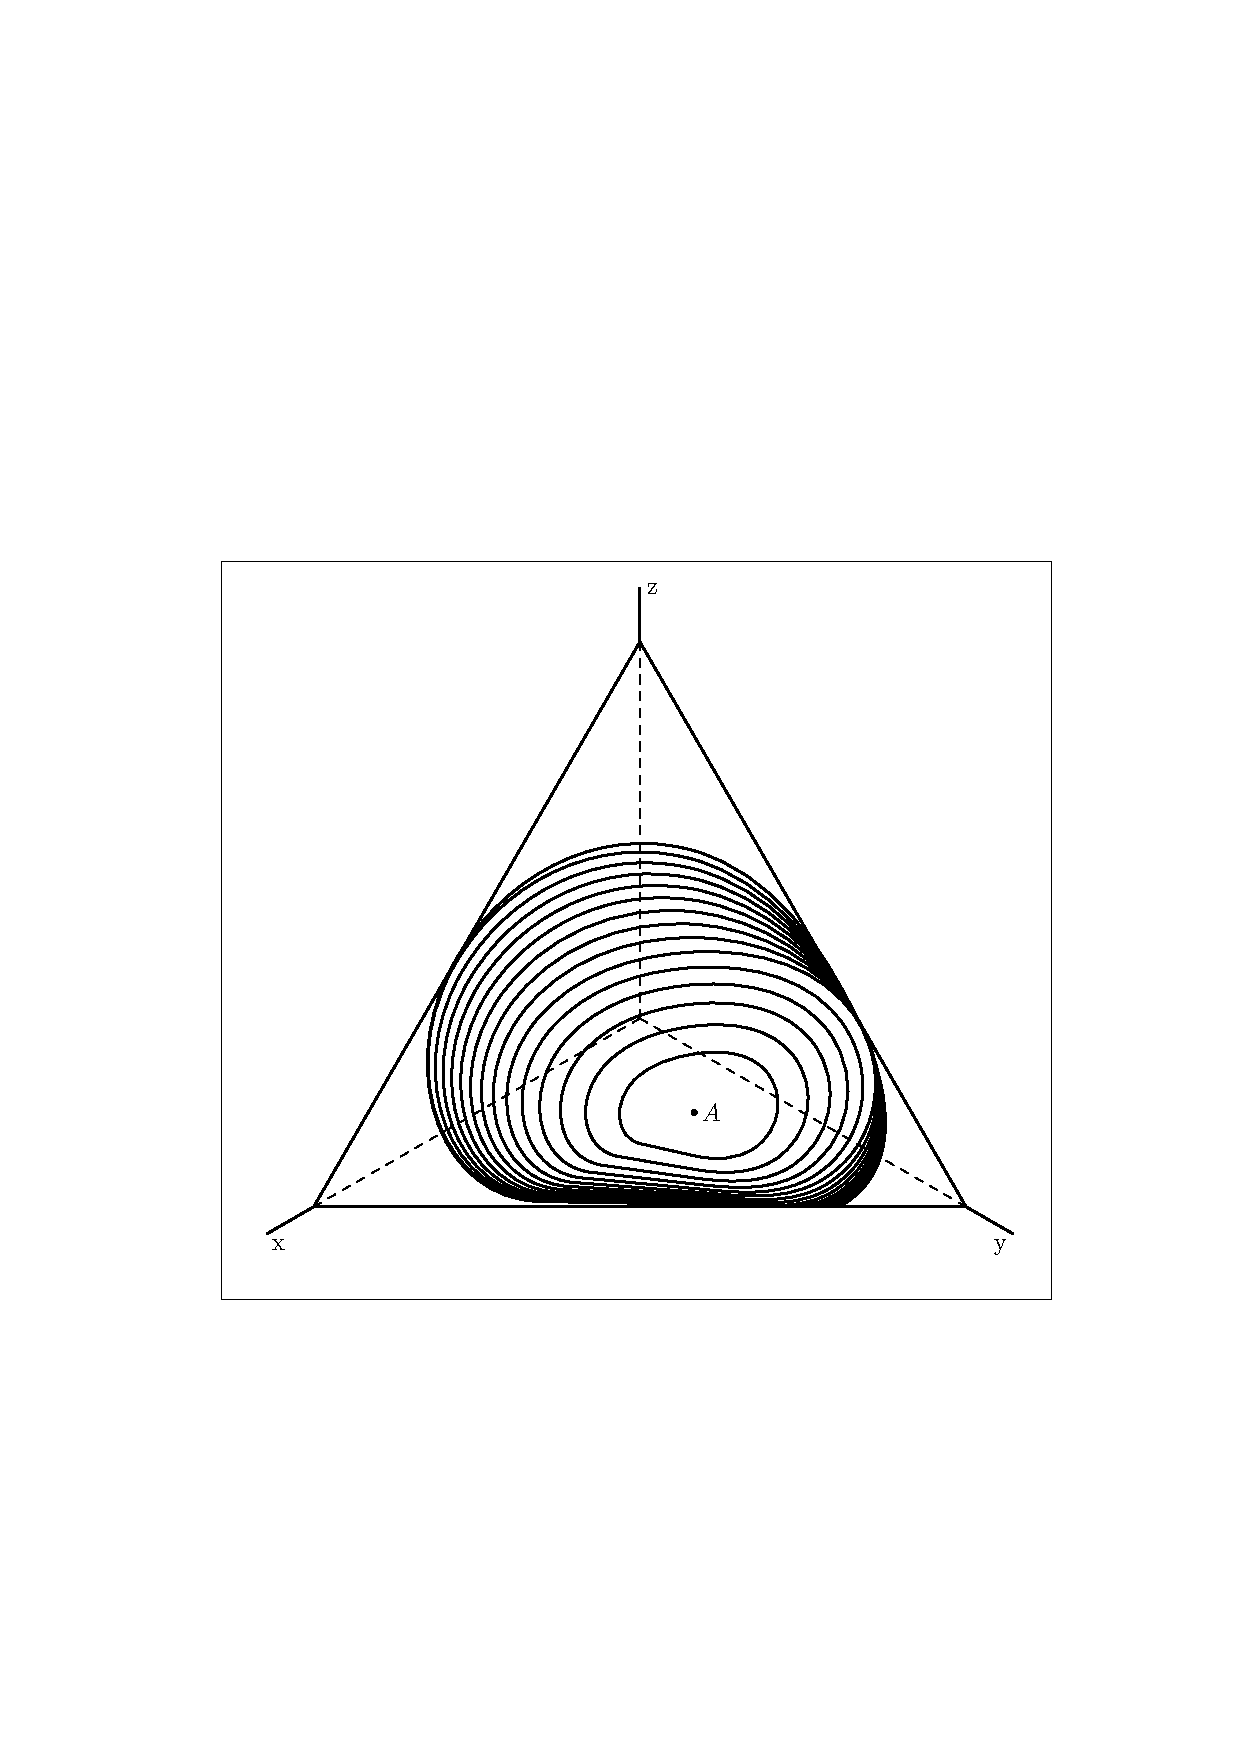
\includegraphics[width=\textwidth]{crj.pdf}
      \caption{\footnotesize The simplex $\mathbb{S}^{3}$ with contour
        lines corresponding to information theory around point $A$ in
        equation (\ref{eq:e6}). Points on the same contour line are
        equidistant from $A$ with respect to the Kullback-Leibler
        divergence. The contrast to figure (\ref{fig:contourslp}) will
        become clear in much more detail in the body of the paper.
        Note that the contour lines of the geometry of reason are
        insensitive to the boundaries of the simplex, while the
        contour lines of information theory reflect them. The main
        argument of this paper is that information theory respects
        epistemic intuitions we have about asymmetry: proximity to
        extreme beliefs with very high or very low probability
        influences the topology that is at the basis of updating.}
      \label{fig:contoursrj}
    \end{minipage}
  \end{flushright}
\end{figure}

\section{Epistemic Utility and the Geometry of Reason}
\label{eugr}

Both Joyce and Leitgeb/Pettigrew propose axioms for a measure of
gradational accuracy for partial beliefs relying on the geometry of
reason, i.e.\ the idea of geometrical distance between distributions
of partial belief expressed in non-negative real numbers. In Joyce,
the geometry of reason is adopted without much reflection. Terms such
as \qnull{midpoint} between two distributions and
$\lambda{}b'+(1-\lambda)b''$ for distributions \qnull{between} two
distributions $b'$ and $b''$ are used freely.

Leitgeb and Pettigrew muse about alternative geometries, especially
non-Euclidean ones. They suspect that these would be based on and in
the end reducible to Euclidean geometry but they do not entertain the
idea that they could drop the requirement of a metric topology
altogether (for the use of non-Euclidean geodesics in statistical
inference see \scite{7}{shunichi85}{}). 

Joyce advocates for axioms such as Weak Convexity and Symmetry in
Euclidean terms, using justifications such as \qeins{the change in
  belief involved in going from $b'$ to $b''$ has the same direction
  but a doubly greater magnitude than change involved in going from
  $b'$ to [the midpoint] $m$} (see \scite{8}{joyce98}{596}). In
subsection \ref{Asymmetry}, I will show that Weak Convexity holds, and
Symmetry does not hold, in \qnull{information geometry.} Information
theory in this context is the topology generated by the
Kullback-Leibler divergence. The term information geometry is due to
Imre Csisz{\'a}r, who considers the Kullback-Leibler divergence an
asymmetric analogue of squared Euclidean distance and derives several
results that are intuitive information geometric counterparts of
standard results in Euclidean geometry (see chapter 3 of
\scite{7}{csiszarshields04}{}).

Leitgeb and Pettigrew's work is continuous with Joyce's work, although
their axioms tend to be stronger including expected inaccuracies. They
show that uniform distribution (a version of the principle of
indifference) requires additional axioms which are much less plausible
than the ones on the basis of which they derive probabilism and
standard conditioning (see \scite{8}{leitgebpettigrew10ii}{250f}); and
that Jeffrey conditioning does not fulfill Joyce's Norm of Gradational
Accuracy (see \scite{8}{joyce98}{579}). Leitgeb and Pettigrew provide
us with an alternative method of updating for Jeffrey-type updating
scenarios, which I will call LP conditioning.

\begin{quotex}
  \beispiel{Sherlock Holmes}\label{ex:holmes} Sherlock Holmes
  attributes the following probabilities to the propositions $E_{i}$
  that $k_{i}$ is the culprit in a crime:
  $P(E_{1})=1/3,P(E_{2})=1/2,P(E_{3})=1/6$, where $k_{1}$ is Mr.\ R.,
  $k_{2}$ is Ms.\ S., and $k_{3}$ is Ms.\ T. Then Holmes finds some
  evidence which convinces him that $P'(F^{*})=1/2$, where $F^{*}$ is
  the proposition that the culprit is male and $P$ is relatively prior
  to $P'$. What should be Holmes' updated probability that Ms.\ S. is
  the culprit?
\end{quotex}

I will look at the recommendations of Jeffrey conditioning and LP
conditioning for example \ref{ex:holmes} in the next section. For now,
we note that LP conditioning violates all of the following seven
plausible expectations for an amujus, an \qnull{alternative method of
  updating for Jeffrey-type updating scenarios.}

\begin{itemize}
\item \textsc{continuity} An amujus ought to be continuous with
  standard conditioning as a limiting case.
\item \textsc{regularity} An amujus ought not to assign a posterior
  probability of $0$ to an event which has a positive prior
  probability and about which the intervening evidence says nothing
  except that a strictly weaker event has a positive posterior
  probability.
\item \textsc{levinstein} An amujus ought not to give \qeins{extremely
    unattractive} results in a Levinstein scenario (see
  \scite{7}{levinstein12}{}).
\item \textsc{invariance} An amujus ought to be partition invariant.
\item \textsc{horizon} An amujus ought to exhibit the horizon effect
  which makes probability distributions which are nearer to extreme
  probability distributions appear to be closer to each other than
  they really are.
\item \textsc{confirmation} An amujus ought to align with intuitions
  we have about degrees of confirmation.
\item \textsc{asymmetry} An amujus ought to reflect epistemic
  asymmetries. Updating from one probability distribution to another
  may need to be reflected in a different proximity relation than
  going the opposite way.
\end{itemize}

We are faced with the choice of rejecting the geometry of reason or
accepting these unpleasant consequences. Fortunately, there is a live
alternative to the geometry of reason: information theory. Information
theory has its own axiomatic approach to justifying probabilism and
standard conditioning (see \scite{7}{shorejohnson80}{}). Furthermore,
information theory provides a justification for Jeffrey conditioning
and generalizes it (see \scite{7}{lukits15}{}). Information theory is
not a geometry of reason because it measures divergences, not
distances, between distributions of partial belief. The divergence of
$b''$ from $b'$ may not be equal to the divergence of $b'$ from $b''$.
Updating methods based on information theory (standard conditioning,
Jeffrey conditioning, the principle of maximum entropy) fulfill
the seven expectations.

The next section provides a simple example where the distance of
geometry and the divergence of information theory differ. With this
difference in mind, I will show how LP conditioning fails the seven
expectations outlined above. The conclusion is that a rational agent
uses information theory, not the geometry of reason.

\section{Geometry of Reason versus Information Theory}
\label{grit}

Consider the following three points in three-dimensional space: 

\begin{equation}
  \label{eq:e6}
    A=\left(\frac{1}{3},\frac{1}{2},\frac{1}{6}\right) \hspace{.5in}
    B=\left(\frac{1}{2},\frac{3}{8},\frac{1}{8}\right)  \hspace{.5in}
    C=\left(\frac{1}{2},\frac{5}{12},\frac{1}{12}\right)
\end{equation}

All three are elements of the three-dimensional simplex
$\mathbb{S}^{3}$: their coordinates add up to $1$. Thus they represent
probability distributions over a partition of the event space into
three events. Now call $D_{\mbox{\tiny KL}}(A,B)$ the Kullback-Leibler
divergence of $A$ from $B$ defined as follows, where $a_{i}$ are the
Cartesian coordinates of $A$:

\begin{equation}
  \label{eq:e7}
  D_{\mbox{\tiny KL}}(A,B)=\sum_{i=1}^{3}a_{i}\ln\frac{a_{i}}{b_{i}}
\end{equation}

The Euclidean distance $\|A-B\|$ is defined as 

\begin{equation}
  \label{eq:e3}
  \sqrt{\sum_{i=1}^{3}\left(a_{i}-b_{i}\right)^{2}}.
\end{equation}

What is remarkable about the three points in (\ref{eq:e6}) is that

\begin{equation}
  \label{eq:e8}
  \|A-C\|\approx{}0.204<\|A-B\|\approx{}0.212
\end{equation}

and

\begin{equation}
  \label{eq:e9}
  D_{\mbox{\tiny KL}}(A,B)\approx{}0.057<D_{\mbox{\tiny KL}}(A,C)\approx{}0.072.
\end{equation}

The Kullback-Leibler divergence and Euclidean distance give different
recommendations with respect to proximity (for illustration see figure
\ref{fig:threepoints}). If $A$ corresponds to my prior and my evidence
is such that I must change the first coordinate to $1/2$ and nothing
stronger, then information theory via the Kullback-Leibler divergence
recommends the posterior corresponding to $B$, whereas the geometry of
reason recommends the posterior corresponding to $C$.

\begin{figure}[ht]
  \begin{flushright}
    \begin{minipage}[h]{.7\linewidth}
      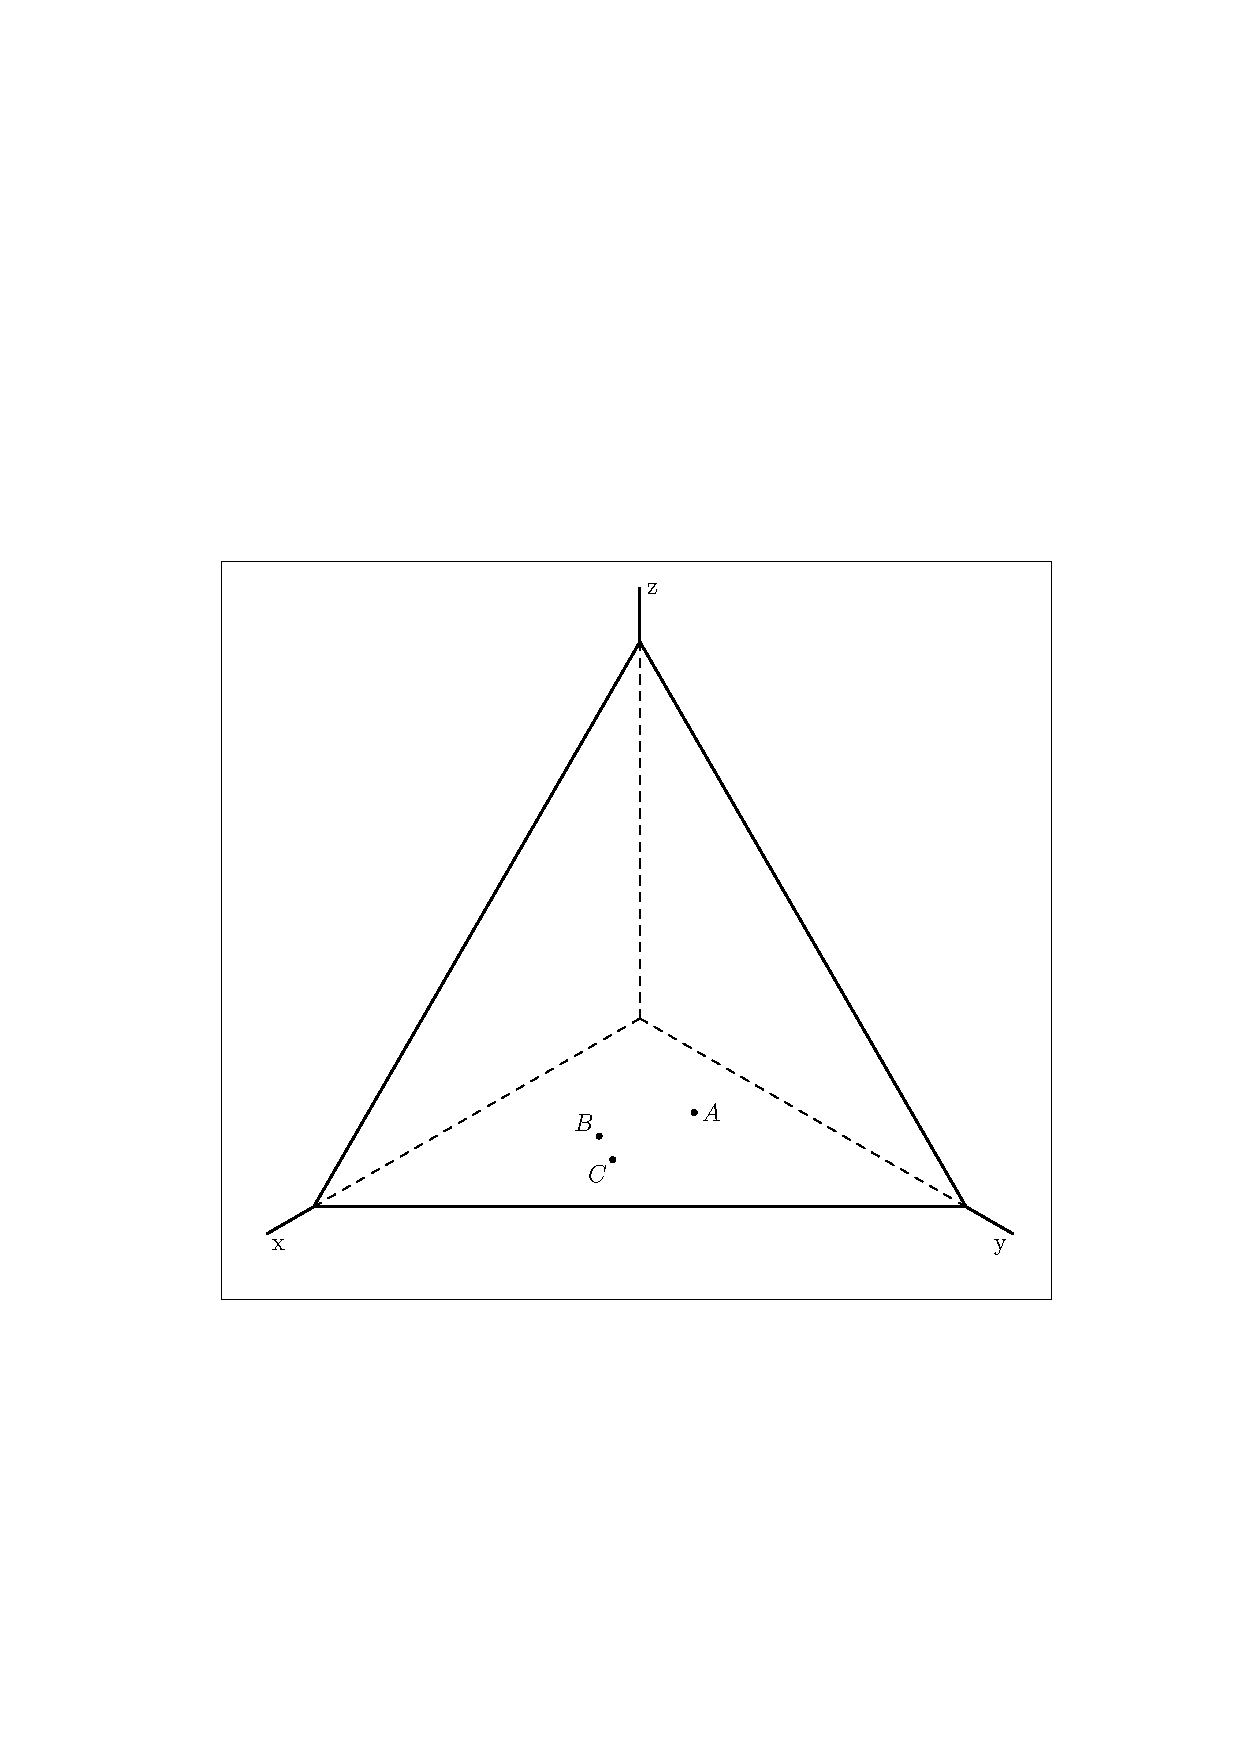
\includegraphics[width=\textwidth]{threepoints.pdf}
      \caption{\footnotesize The simplex $\mathbb{S}^{3}$ in
        three-dimensional space $\mathbb{R}^{3}$ with points $A,B,C$
        as in equation (\ref{eq:e6}). Note that geometrically speaking
        $C$ is closer to $A$ than $B$ is. Using the Kullback-Leibler
        divergence, however, $B$ is closer to $A$ than $C$ is. The
        reason is asymmetry in information theory, which accords with
        our intuitions about epistemic space.}
      \label{fig:threepoints}
    \end{minipage}
  \end{flushright}
\end{figure}

Here is a brief outline how Leitgeb and Pettigrew arrive at posterior
probability distributions in Jeffrey-type updating scenarios, using
their invariance criterion with respect to global and local
inaccuracy. I will call their method LP conditioning.

\begin{quotex}
  \beispiel{Abstract Holmes}\label{ex:abstract} Consider a possibility
  space $W=E_{1}\cup{}E_{2}\cup{}E_{3}$ (the $E_{i}$ are sets of
  states which are pairwise disjoint and whose union is $W$) and a
  partition $\mathcal{F}$ of $W$ such that
  $\mathcal{F}=\{F^{*},F^{**}\}=\{E_{1},E_{2}\cup{}E_{3}\}$.
\end{quotex}

Let $P$ be the prior probability function on $W$ and $P'$ the
posterior. I will keep the notation informal to make this simple, not
mathematically precise. Jeffrey-type updating scenarios give us new
information on the posterior probabilities of partitions such as
$\mathcal{F}$. In example \ref{ex:abstract}, let

\begin{equation}
  \label{eq:priors}
  \begin{array}{rcl}
    P(E_{1})&=&1/3 \\
    P(E_{2})&=&1/2 \\
    P(E_{3})&=&1/6
  \end{array}
\end{equation}

and the new evidence constrain $P'$ such that
$P'(F^{*})=1/2=P'(F^{**})$.

Jeffrey conditioning works on the intuition that the posterior
probabilities conditional on the partition elements equal the prior
probabilities conditional on the partition elements (since we have no
information in the evidence that they should have changed):

\begin{align}
  \label{eq:jc}
  &P'_{\mbox{\tiny JC}}(E_{i})&=&P'(E_{i}|F^{*})P'(F^{*})+P'(E_{i}|F^{**})P'(F^{**})\notag \\
  &&=&P(E_{i}|F^{*})P'(F^{*})+P(E_{i}|F^{**})P'(F^{**})
\end{align}

Jeffrey conditioning is controversial (for an introduction to Jeffrey
conditioning see \scite{7}{jeffrey65}{}; for its statistical and
formal properties see \scite{7}{diaconiszabell82}{}; for a pragmatic
vindication of Jeffrey conditioning see \scite{7}{armendt80}{}, and
\scite{7}{skyrms86}{}; for criticism see
\scite{7}{howsonfranklin94}{}). Information theory, however, supports
Jeffrey conditioning. 

Leitgeb and Pettigrew show that Jeffrey conditioning does not in
general pick out the minimally inaccurate posterior probability
distribution. If the geometry of reason as presented in Leitgeb and
Pettigrew is sound, this would constitute a powerful criticism of
Jeffrey conditioning. Leitgeb and Pettigrew introduce an alternative
to Jeffrey conditioning, which we have called LP conditioning. It
proceeds as follows for example \ref{ex:abstract} and in general
provides the minimally inaccurate posterior probability distribution
in Jeffrey-type updating scenarios.

Solve the following two equations for $x$ and $y$:

\begin{equation}
  \label{eq:lpce}
  \begin{array}{rcl}
    P(E_{1})+x&=&P'(F^{*}) \\
    P(E_{2})+y+P(E_{3})+y&=&P'(F^{**})
  \end{array}
\end{equation}

and then set

\begin{equation}
  \label{eq:lpcf}
  \begin{array}{rcl}
    P'_{\mbox{\tiny LP}}(E_{1})&=&P(E_{1})+x \\
    P'_{\mbox{\tiny LP}}(E_{2})&=&P(E_{2})+y \\
    P'_{\mbox{\tiny LP}}(E_{3})&=&P(E_{3})+y
  \end{array}
\end{equation}

For the more formal and more general account see
\scite{8}{leitgebpettigrew10ii}{254}. The results for example
\ref{ex:abstract} are:

\begin{equation}
  \label{eq:lpcres}
  \begin{array}{rcl}
    P'_{\mbox{\tiny LP}}(E_{1})&=&1/2 \\
    P'_{\mbox{\tiny LP}}(E_{2})&=&5/12 \\
    P'_{\mbox{\tiny LP}}(E_{3})&=&1/12
  \end{array}
\end{equation}

Compare these results to the results of Jeffrey conditioning:

\begin{equation}
  \label{eq:jcres}
  \begin{array}{rcl}
    P'_{\mbox{\tiny JC}}(E_{1})&=&1/2 \\
    P'_{\mbox{\tiny JC}}(E_{2})&=&3/8 \\
    P'_{\mbox{\tiny JC}}(E_{3})&=&1/8
  \end{array}
\end{equation}

Note that (\ref{eq:priors}), (\ref{eq:jcres}), and (\ref{eq:lpcres})
correspond to $A,B,C$ in (\ref{eq:e6}). 

\section{Seven Expectations}
\label{fivex}

It remains to provide more detail for the seven expectations and to
show how LP conditioning violates them. The subsections on
\textsc{confirmation}, \textsc{horizon}, and \textsc{asymmetry} have
been abridged to accommodate the word limit for this submission. The
full-length paper contains the complete version of these arguments.

\subsection{Continuity}
\label{Continuity}

LP conditioning violates \textsc{continuity} because standard
conditioning gives a different recommendation than a parallel sequence
of Jeffrey-type updating scenarios which get arbitrarily close to
standard event observation. This is especially troubling considering
how important the case for standard conditioning is to Leitgeb and
Pettigrew.

To illustrate a \textsc{continuity} violation, consider the case where
Sherlock Holmes reduces his credence that the culprit was male to
$\varepsilon_{n}=1/n$ for $n=4,5,\ldots$. The sequence
$\varepsilon_{n}$ is not meant to reflect a case where Sherlock Holmes
becomes successively more certain that the culprit was female. It is
meant to reflect countably many parallel scenarios which only differ
by the degree to which Sherlock Holmes is sure that the culprit was
female. These parallel scenarios give rise to a parallel sequence (as
opposed to a successive sequence) of updated probabilities
$P'_{\mbox{\tiny LP}}(F^{**})$ and another sequence of updated
probabilities $P'_{\mbox{\tiny JC}}(F^{**})$ ($F^{**}$ is the
proposition that the culprit is female). As $n\rightarrow\infty$, both
of these sequences go to one.

Straightforward conditionalization on the evidence that \qnull{the
  culprit is female} gives us 

\begin{equation}
  \label{eq:sherlockcontsc}
  \begin{array}{rcl}
  P'_{\mbox{\tiny SC}}(E_{1})&=&0\\
  P'_{\mbox{\tiny SC}}(E_{2})&=&3/4\\
  P'_{\mbox{\tiny SC}}(E_{3})&=&1/4.
\end{array}
\end{equation}

Letting $n\rightarrow\infty$ for Jeffrey conditioning yields

\begin{equation}
  \label{eq:sherlockcontjc}
  \begin{array}{rcccl}
  P'_{\mbox{\tiny JC}}(E_{1})&=&1/n&\rightarrow&0\\
  P'_{\mbox{\tiny JC}}(E_{2})&=&3(n-1)/4n&\rightarrow&3/4\\
  P'_{\mbox{\tiny JC}}(E_{3})&=&(n-1)/4n&\rightarrow&1/4,
\end{array}
\end{equation}

whereas letting $n\rightarrow\infty$ for LP conditioning yields

\begin{equation}
  \label{eq:sherlockcontlp}
  \begin{array}{rcccl}
  P'_{\mbox{\tiny LP}}(E_{1})&=&1/n&\rightarrow&0\\
  P'_{\mbox{\tiny LP}}(E_{2})&=&(4n-1)/6n&\rightarrow&2/3\\
  P'_{\mbox{\tiny LP}}(E_{3})&=&(2n-1)/6n&\rightarrow&1/3.
\end{array}
\end{equation}

LP conditioning violates \textsc{continuity}.

\subsection{Regularity}
\label{Regularity}

LP conditioning violates \textsc{regularity} because formerly positive
probabilities can be reduced to $0$ even though the new information in
the Jeffrey-type updating scenario makes no such requirements (as is
usually the case for standard conditioning). Ironically, Jeffrey-type
updating scenarios are meant to be a better reflection of real-life
updating because they avoid extreme probabilities. 

The violation becomes especially egregious if we are already somewhat
sympathetic to an information-based account: the amount of information
required to turn a non-extreme probability into one that is extreme
($0$ or $1$) is infinite. Whereas the geometry of reason considers
extreme probabilities to be easily accessible by non-extreme
probabilities under new information (much like a marble rolling off a
table or a bowling ball heading for the gutter), information theory
envisions extreme probabilities more like an event horizon. The nearer
you are to the extreme probabilities, the more information you need to
move on. For an observer, the horizon is never reached.

\begin{quotex}
  \beispiel{Regularity Holmes}\label{ex:regularity} Everything is as
  in example \ref{ex:holmes}, except that Sherlock Holmes becomes
  confident to a degree of $2/3$ that Mr.\ R is the culprit and
  updates his relatively prior probability distribution in
  (\ref{eq:priors}).
\end{quotex}

Then his posterior probabilities look as follows:

\begin{equation}
  \label{eq:sherlockposteriorjcreg}
  \begin{array}{rcl}
  P'_{\mbox{\tiny JC}}(E_{1})&=&2/3\\
  P'_{\mbox{\tiny JC}}(E_{2})&=&1/4\\
  P'_{\mbox{\tiny JC}}(E_{3})&=&1/12
\end{array}
\end{equation}

\begin{equation}
  \label{eq:sherlockposteriorlpreg}
  \begin{array}{rcl}
  P'_{\mbox{\tiny LP}}(E_{1})&=&2/3\\
  P'_{\mbox{\tiny LP}}(E_{2})&=&1/3\\
  P'_{\mbox{\tiny LP}}(E_{3})&=&0
\end{array}
\end{equation}

With LP conditioning, Sherlock Holmes' subjective probability that
Ms.\ T is the culprit in example \ref{ex:regularity} has been reduced
to zero. No finite amount of information could bring Ms.\ T back into
consideration as a culprit in this crime, and Sherlock Holmes should
be willing to bet any amount of money against a penny that she is not
the culprit---even though his evidence is nothing more than an
increase in the probability that Mr.\ R is the culprit (see
(\ref{fig:threepointshat} for illustration).

\begin{figure}[ht]
  \begin{flushright}
    \begin{minipage}[h]{.7\linewidth}
      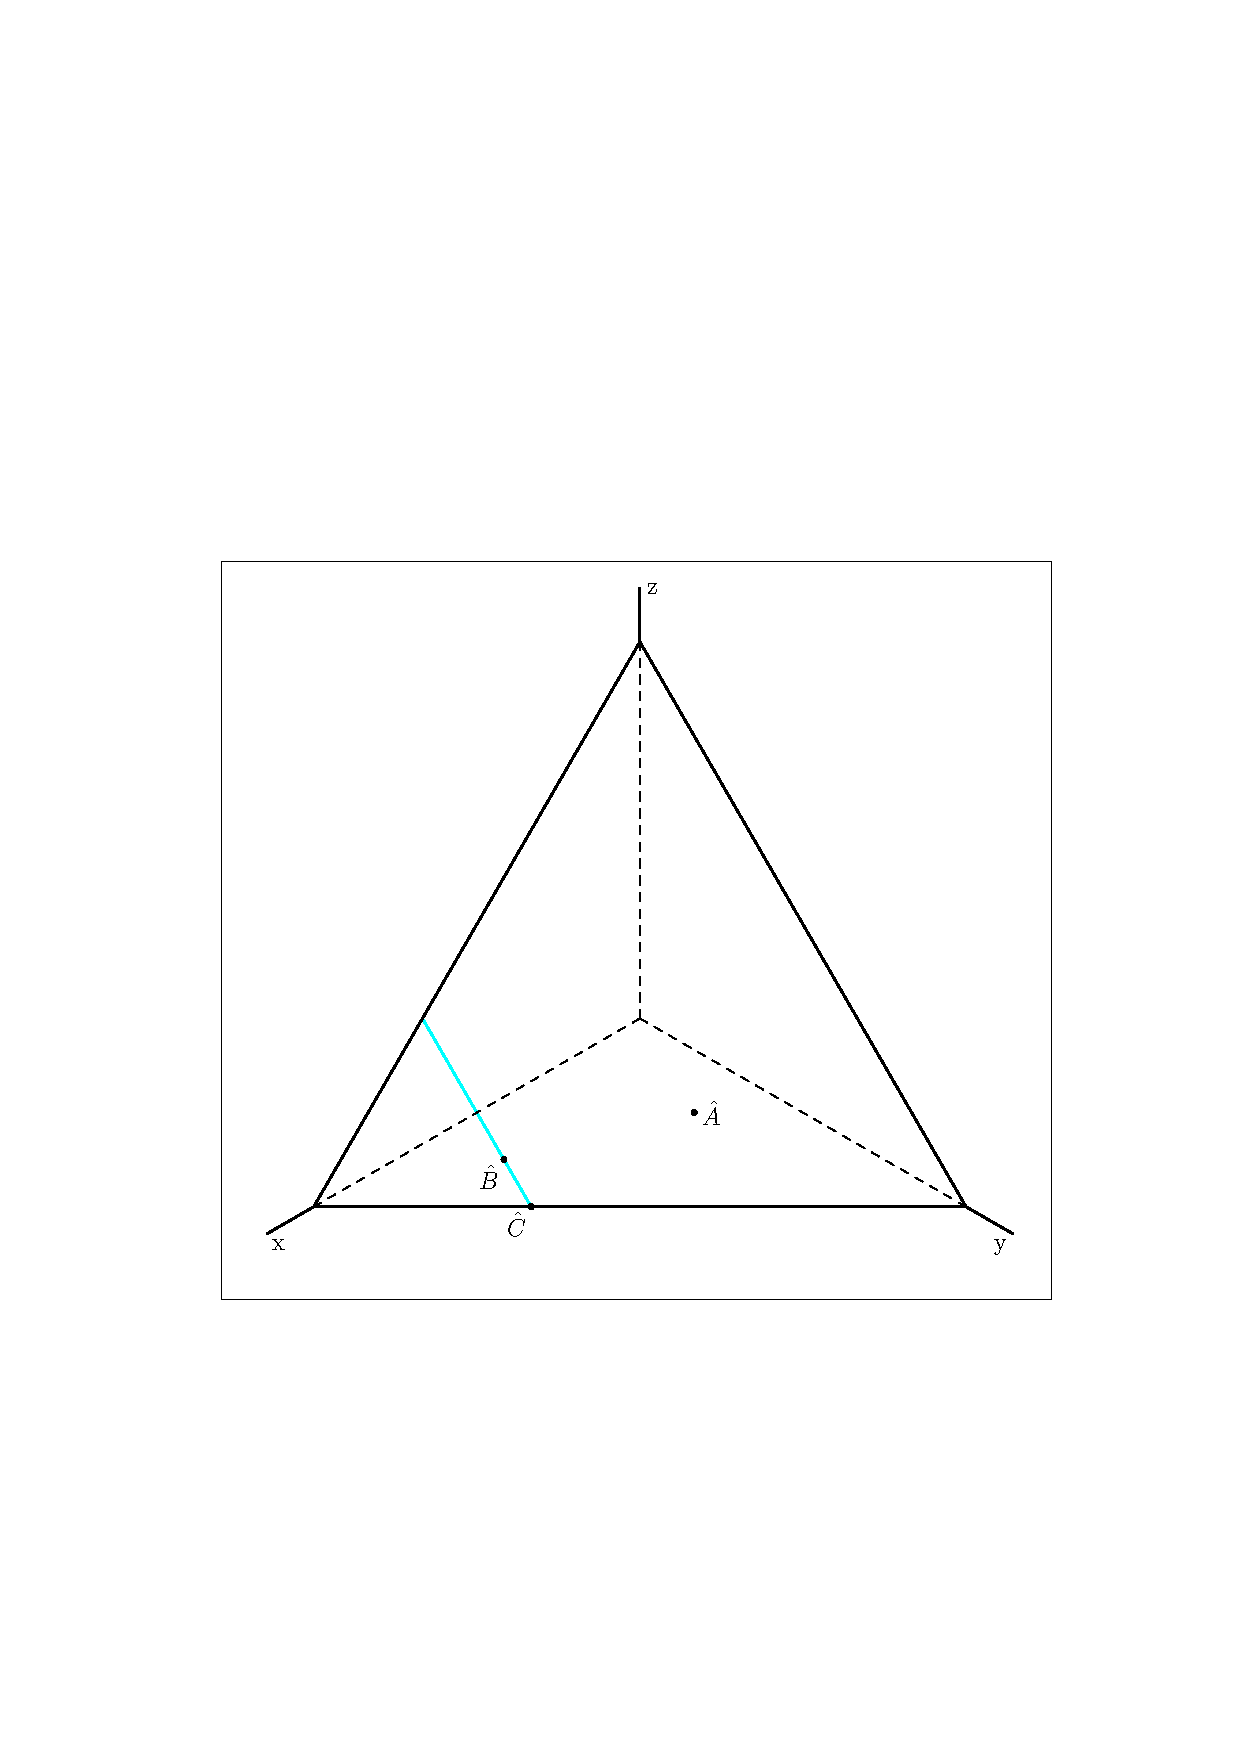
\includegraphics[width=\textwidth]{threepointshat.pdf}
      \caption{\footnotesize The simplex $\mathbb{S}^{3}$ in
        three-dimensional space $\mathbb{R}^{3}$ with points
        $\hat{A},\hat{B},\hat{C}$ corresponding to the probability
        distributions in (\ref{eq:priors}),
        (\ref{eq:sherlockposteriorjcreg}), and
        (\ref{eq:sherlockposteriorlpreg}). Similar to figure
        (\ref{fig:threepoints}), $\hat{C}$ is closer to $\hat{A}$ than
        $\hat{B}$ is, geometrically speaking. Using the
        Kullback-Leibler divergence, however, $\hat{B}$ is closer to
        $\hat{A}$ than $\hat{C}$ is. The probability distribution
        corresponding to $\hat{B}$ is the Jeffrey posterior with
        respect to the probability distribution corresponding to
        $\hat{A}$. The probability distribution corresponding to
        $\hat{C}$ is the LP posterior and contains an extreme element.
        Jeffrey conditioning, by regularity, avoids extreme
        probabilities not required by the evidence. The coloured line
        going through $\hat{B}$ and $\hat{C}$ signifies the constraint
        that the evidence imposes on the posterior distribution,
        mandating that the $x$-coordinate must be $2/3$.}
      \label{fig:threepointshat}
    \end{minipage}
  \end{flushright}
\end{figure}

LP conditioning violates \textsc{regularity}.

\subsection{Levinstein}
\label{Levinstein}

LP conditioning violates \textsc{levinstein} because of \qeins{the
  potentially dramatic effect [LP conditioning] can have on the
  likelihood ratios between different propositions}
\scite{3}{levinstein12}{419}. Consider Benjamin Levinstein's example:

\begin{quotex}
  \beispiel{Levinstein's Ghost}\label{ex:levinstein} There is a car
  behind an opaque door, which you are almost sure is blue but which
  you know might be red. You are almost certain of materialism, but
  you admit that there's some minute possibility that ghosts exist.
  Now the opaque door is opened, and the lighting is fairly good. You
  are quite surprised at your sensory input: your new credence that
  the car is red is very high.
\end{quotex}

Jeffrey conditioning leads to no change in opinion about ghosts. Under
LP conditioning, however, seeing the car raises the probability that
there are ghosts to an astonishing 47\%, given Levinstein's reasonable
priors. Levinstein proposes a logarithmic inaccuracy measure as a
remedy to avoid violation of \textsc{levinstein} (vaguely related to
the Kullback-Leibler divergence), but his account falls far short of
the formal scope, substance, and integrity of information theory.
As a special case of applying a Levinstein-type logarithmic inaccuracy
measure, information theory does not violate \textsc{levinstein}.

\subsection{Invariance}
\label{Invariance}

LP conditioning violates \textsc{invariance} because two agents who
have identical credences with respect to a partition of the event
space may disagree about this partition after LP conditioning, even
when the Jeffrey-type updating scenario provides no new information
about the more finely grained partitions on which the two agents
disagree. 

\begin{quotex}
  \beispiel{Jane Marple}\label{ex:marple} Jane Marple is on the same
  case as Sherlock Holmes in example \ref{ex:holmes} and arrives at
  the same relatively prior probability distribution as Sherlock
  Holmes (we will call Jane Marple's relatively prior probability
  distribution $Q$ and her posterior probability distribution $Q'$).
  Jane Marple, however, has a more fine-grained probability assignment
  than Sherlock Holmes and distinguishes between the case where Ms.\ S
  went to boarding school with her, of which she has a vague memory,
  and the case where Ms.\ S did not and the vague memory is only about
  a fleeting resemblance of Ms.\ S with another boarding school mate.
  Whether or not Ms.\ S went to boarding school with Jane Marple is
  completely beside the point with respect to the crime, and Jane
  Marple considers the possibilities equiprobable whether or not Ms.\
  S went to boarding school with her.
\end{quotex}

Let $E_{2}\equiv{}E_{2}^{*}\vee{}E_{2}^{**}$, where $E_{2}^{*}$ is the
proposition that Ms.\ S is the culprit and she went to boarding school
with Jane Marple and $E_{2}^{**}$ is the proposition that Ms.\ S is
the culprit and she did not go to boarding school with Jane Marple.
Then

\begin{equation}
  \label{eq:marpleprior}
  \begin{array}{rcl}
  Q(E_{1})&=&1/3\\
  Q(E_{2}^{*})&=&1/4\\
  Q(E_{2}^{**})&=&1/4\\
  Q(E_{3})&=&1/6.
\end{array}
\end{equation}

Now note that while Sherlock Holmes and Jane Marple agree on the
relevant facts of the criminal case (who is the culprit?) in their
posterior probabilities if they use Jeffrey conditioning,

\begin{equation}
  \label{eq:sherlockposteriorjc}
  \begin{array}{rcl}
  P'_{\mbox{\tiny JC}}(E_{1})&=&1/2\\
  P'_{\mbox{\tiny JC}}(E_{2})&=&3/8\\
  P'_{\mbox{\tiny JC}}(E_{3})&=&1/8
\end{array}
\end{equation}

\begin{equation}
  \label{eq:marpleposteriorjc}
  \begin{array}{rcl}
  Q'_{\mbox{\tiny JC}}(E_{1})&=&1/2\\
  Q'_{\mbox{\tiny JC}}(E_{2}^{*})&=&3/16\\
  Q'_{\mbox{\tiny JC}}(E_{2}^{**})&=&3/16\\
  Q'_{\mbox{\tiny JC}}(E_{3})&=&1/8
\end{array}
\end{equation}

they do not agree if they use LP conditioning,

\begin{equation}
  \label{eq:sherlockposteriorlp}
  \begin{array}{rcl}
  P'_{\mbox{\tiny LP}}(E_{1})&=&1/2\\
  P'_{\mbox{\tiny LP}}(E_{2})&=&5/12\\
  P'_{\mbox{\tiny LP}}(E_{3})&=&1/12
\end{array}
\end{equation}

\begin{equation}
  \label{eq:marpleposteriorlp}
  \begin{array}{rcl}
  Q'_{\mbox{\tiny LP}}(E_{1})&=&1/2\\
  Q'_{\mbox{\tiny LP}}(E_{2}^{*})&=&7/36\\
  Q'_{\mbox{\tiny LP}}(E_{2}^{**})&=&7/36\\
  Q'_{\mbox{\tiny LP}}(E_{3})&=&1/9.
\end{array}
\end{equation}

LP conditioning violates \textsc{invariance}.

\subsection{Horizon}
\label{Horizon}

\begin{quotex}
  \beispiel{Undergraduate Complaint}\label{ex:complaint} An
  undergraduate student complains to the department head that the
  professor will not reconsider an 89\% grade (which misses an A+ by
  one percent) when reconsideration was given to other students with a
  67\% grade (which misses a B- by one percent).
\end{quotex}

Intuitions may diverge, but the professor's reasoning is as follows.
To improve a 60\% paper by ten percent is easily accomplished: having
your roommate check your grammar, your spelling, and your line of
argument will sometimes do the trick. It is incomparably more
difficult to improve an 85\% paper by ten percent: it may take doing a
PhD to turn a student who writes the former into a student who writes
the latter. Consequently, the step from 89\% to 90\% is much greater
than the step from 67\% to 68\%.

The emphasis in this argument is on distance, not confirmation, but
the next subsection can be considered to be a special case of
\textsc{horizon}. LP conditioning violates \textsc{horizon} because it
ignores the epistemic intuition that proximity relations near extreme
probabilities are different than away from them (more central rather
than peripheral). It should be noted that there are non-Euclidean
metrics that obey both \textsc{horizon} and \textsc{confirmation}.

\subsection{Confirmation}
\label{Confirmation}

From an epistemic perspective, updating towards extreme probabilities
should become increasingly difficult. Once a hypothesis is already
considered to be highly likely or highly unlikely, confirmation or
disconfirmation is much harder to come by than in the case of
near-equiprobability between alternative hypotheses. The geometry of
reason ignores this analogy from confirmation theory; information
theory reflects it.

David Christensen's account of degree of confirmation, for example,
shows how $S$-support given by $E$ is stable over Jeffrey conditioning
on $\{E,\urcorner{}E\}$, which is not the case for LP-conditioning
(see \scite{8}{christensen99}{451}). LP conditioning violates
\textsc{confirmation}.

\subsection{Asymmetry}
\label{Asymmetry}

Asymmetry presents a problem for the geometry of reason as well as for
information theory. For the geometry of reason, the problem is akin to
\textsc{continuity}. For information theory, the problem is the
non-trivial nature of the asymmetries it induces, which somehow need
to be reconnected to epistemic justification. I will consider this
problem in a moment, but first I will have a look at the problem for
the geometry of reason.

Even the scrupulous about partial beliefs (such as Isaac Levi) concede
that extreme probabilities are special and create asymmetries in
updating: moving in direction from certainty to uncertainty is
asymmetrical to moving in direction from uncertainty to certainty.
Geometry of reason's metric topology, however, allows for no
asymmetries.

The asymmetry is obvious when extreme probabilities are in play.

\begin{quotex}
  \beispiel{Extreme Asymmetry}\label{ex:extreme} Consider two cases
  where for case 1 the prior probabilities are
  $P(Y_{1})=0.4,P(Y_{2})=0.3,P(Y_{3})=0.3$ and the posterior
  probabilities are $P'(Y_{1})=0,P'(Y_{2})=0.5,P'(Y_{3})=0.5$; for
  case 2 the prior probabilities are
  $Q(Y_{1})=0,Q(Y_{2})=0.5,Q(Y_{3})=0.5$ and the posterior
  probabilities are $Q'(Y_{1})=0.4,Q'(Y_{2})=0.3,Q'(Y_{3})=0.3$;
\end{quotex}

Case 1 is a straightforward application of standard conditioning. Case
2 is much more complicated: what does it take to raise a prior
probability of zero to a positive number? In terms of information
theory, the information required is infinite. Case 2 is also not
compatible with standard conditioning (at least not with what Alan
H{\'a}jek calls the ratio analysis of conditional probability, see
\scite{7}{hajek03}{}). The geometry of reason may want to solve this
problem by signing on to a version of regularity, but then it may be
exposed to violating \textsc{regularity}.

Consider now the problem for information theory. Given the asymmetric
similarity measure of probability distributions that information
theory requires (the Kullback-Leibler divergence), a prior probability
distribution $P$ may be closer to a posterior probability distribution
$Q$ than $Q$ is to $P$ if their roles (prior-posterior) are reversed.
That is just what we would expect. The problem is that there is
another posterior probability distribution $R$ where the situation is
just the opposite: prior $P$ is further away from posterior $R$ than
prior $R$ is from posterior $P$. And whether a probability
distribution different from $P$ is of the $Q$-type or of the $R$-type
escapes any epistemic intuition.

Let me put this differently to emphasize the gravity of the situation
for information theory. For simplicity, let us consider probability
distributions and their associated credence functions on an event
space with three atoms $\Omega=\{\omega_{1},\omega_{2},\omega_{3}\}$.
The simplex $\mathbb{S}^{3}$ represents all of these probability
distributions. Every point $P$ in $\mathbb{S}^{3}$ representing a
probability distribution induces a partition on $\mathbb{S}^{3}$ into
points that are symmetric to $P$, positively skew-symmetric to $P$,
and negatively skew-symmetric to $P$ given the topology of information
theory.

In other words, if

\begin{equation}
  \label{eq:sksy}
  \Delta_{P}(P')=D_{\mbox{\tiny KL}}(P',P)-D_{\mbox{\tiny KL}}(P,P'),
\end{equation}

then, holding $P$ fixed, $\mathbb{S}^{3}$ is partitioned into three
regions, $\Delta^{-1}(\mathbb{R}_{>0})$ (red in figure
\ref{fig:concat}), $\Delta^{-1}(\mathbb{R}_{<0})$ (blue in figure
\ref{fig:concat}), and $\Delta^{-1}(\{0\})$ (in figure
\ref{fig:concat}, this would be the line between the red and the
blue). One could have a simple epistemic intuition such as \qnull{it
  takes less to update from a more uncertain probability distribution
  to a more certain probability distribution than the reverse
  direction,} where the degree of certainty in a probability
distribution is measured by its entropy. This simple intuition accords
with what we said about extreme probabilities: it is, ignoring
regularity for a moment, information-theoretically acceptable to
update by standard conditionalization, decreasing the entropy; but the
reverse direction is not covered by standard conditionalization and
requires an infinite amount of information (raising a zero probability
to a positive probability).

It turns out that the Kullback-Leibler divergence does not support
this simple intuition. The tripartite partition induced by
(\ref{eq:sksy}) is non-trivial---some probability distributions are of
the $Q$-type (red), some are of the $R$-type (blue), and it is
difficult to think of an epistemic distinction between them that does
not already presuppose information theory. See figure \ref{fig:concat}
for graphical illustration of this point.

\begin{figure}[ht]
  \begin{flushright}
    \begin{minipage}[h]{.82\linewidth}
      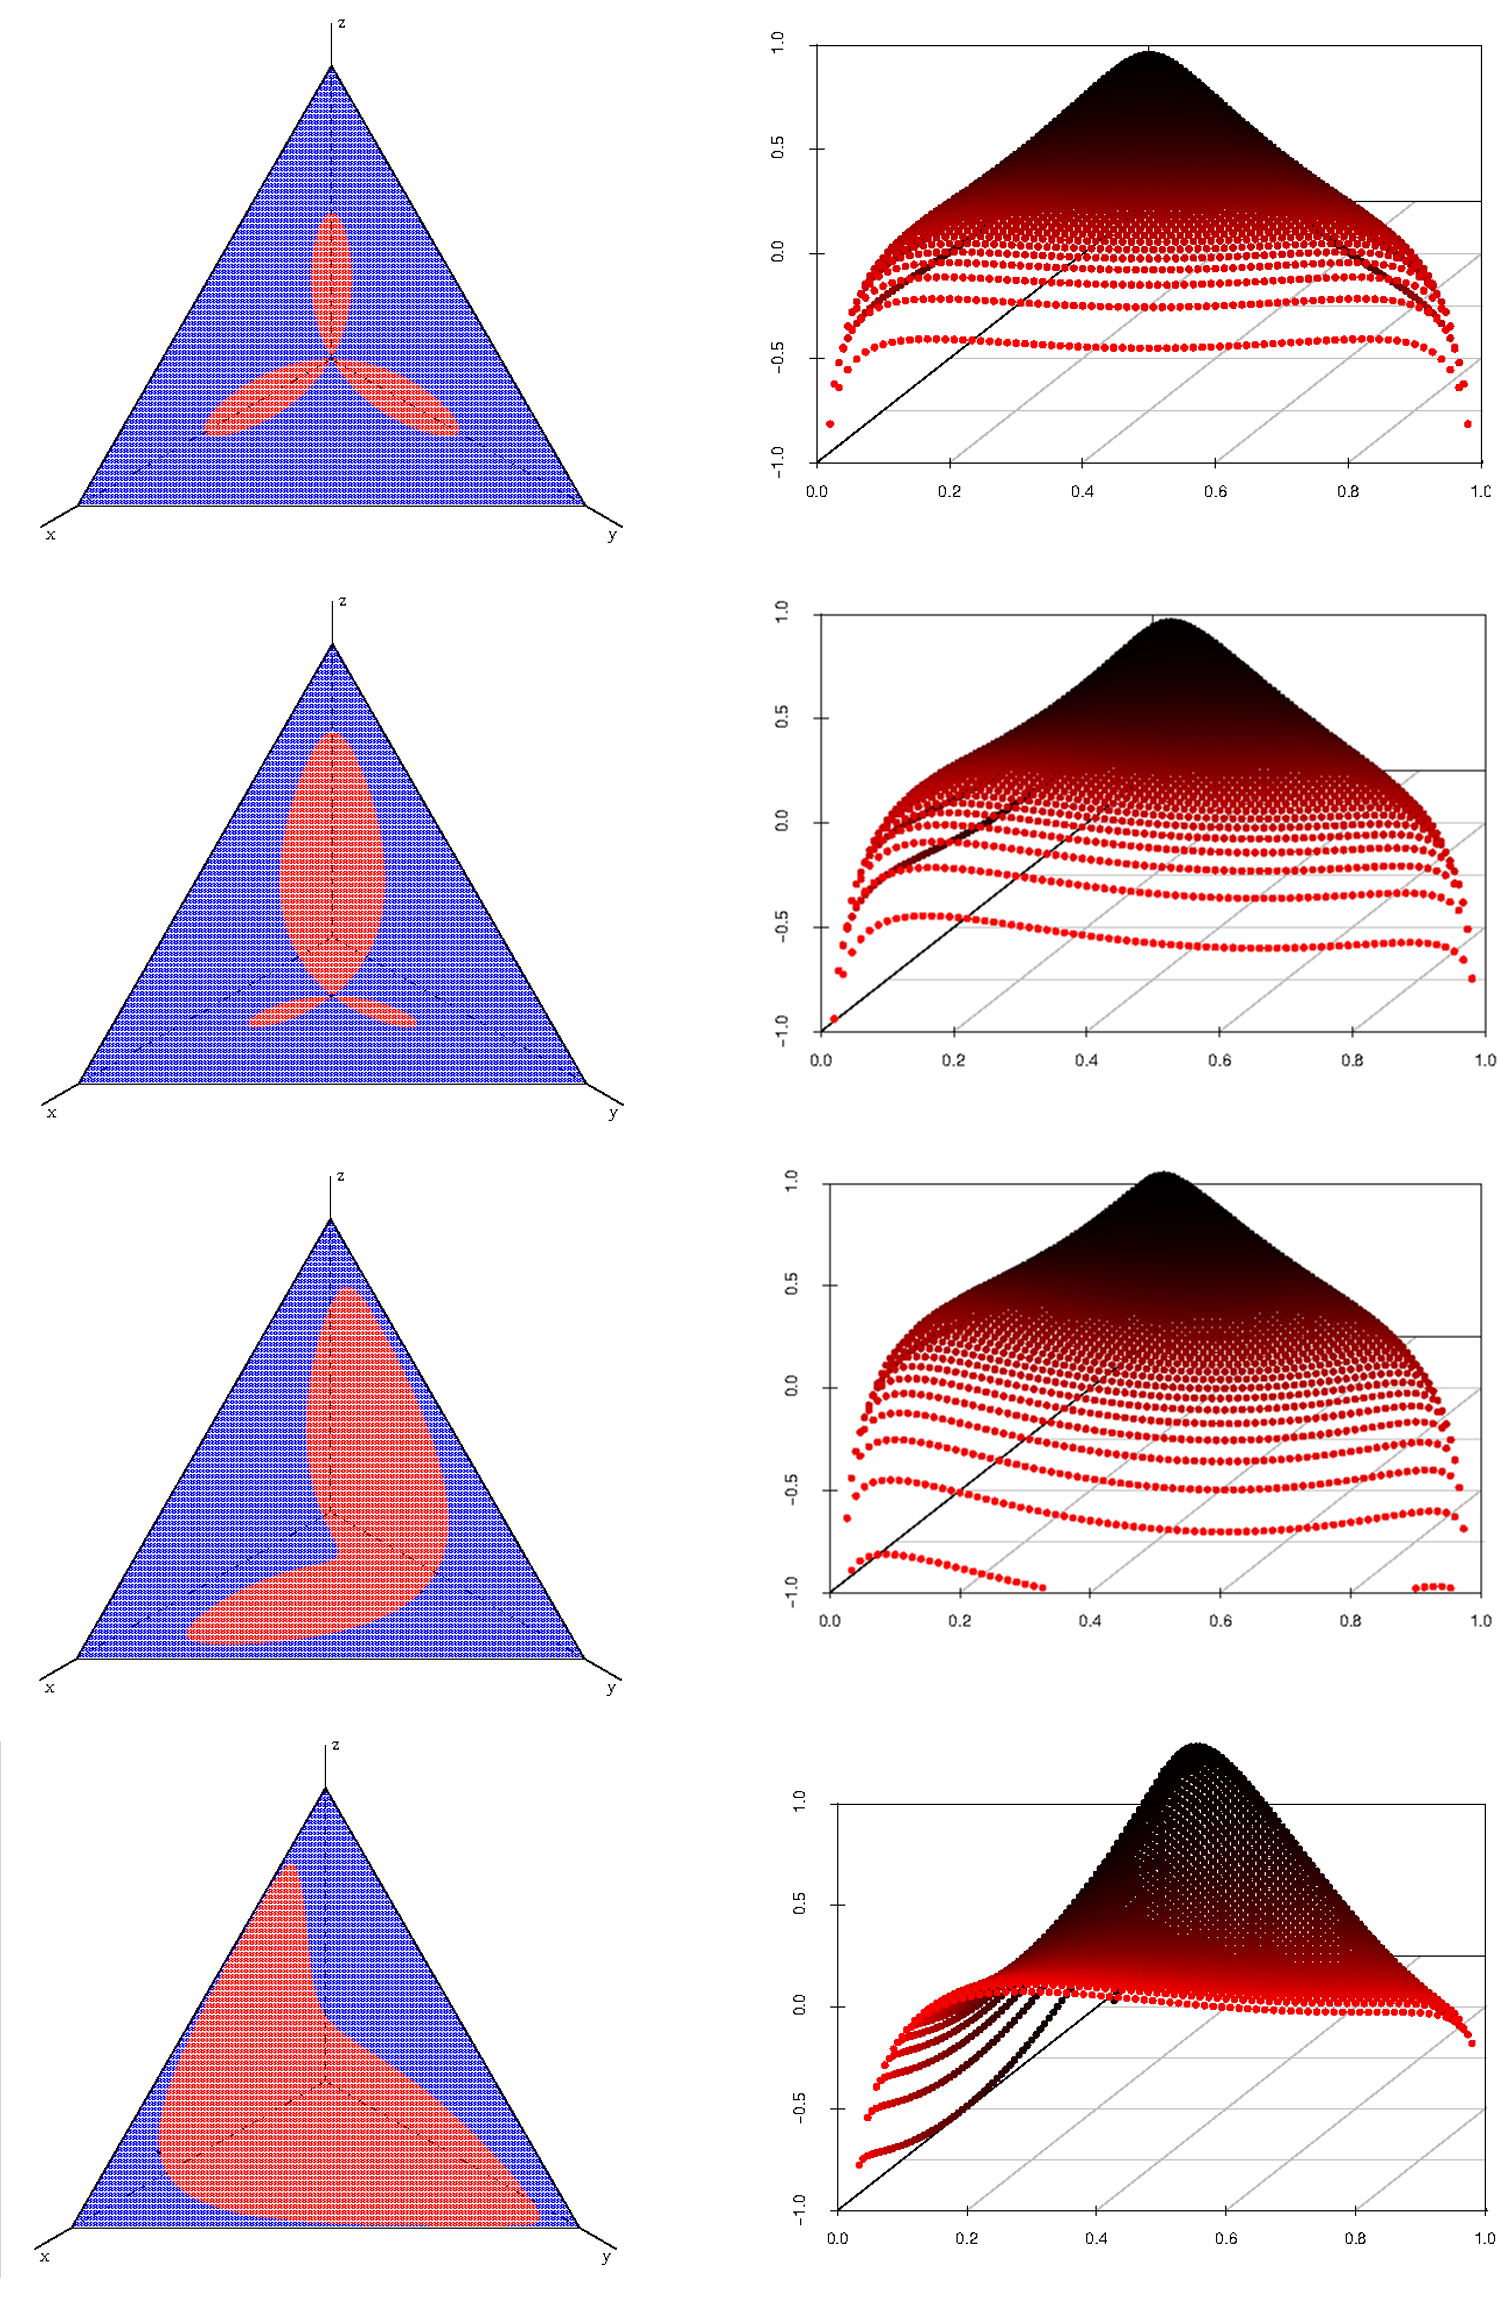
\includegraphics[width=\textwidth]{concat1.png}
      \caption{\footnotesize The partitions induced by equation
        (\ref{eq:sksy}) on the left, corresponding to the 3D
        scatterplot for $\Delta_{P}$ on the right. From top to bottom,
        $P=(1/3,1/3,1/3); P=(0.4,0.4,0.2); P=(0.242,0.604,0.154);
        P=(0.741,0.087,0.172)$.
        Note that for the geometry of reason, the diagrams are
        trivial. The challenge for information theory is to explain
        the non-triviality of these diagrams epistemically without
        begging the question.}
      \label{fig:concat}
    \end{minipage}
  \end{flushright}
\end{figure}

This paper has no solution for the problem which non-question-begging
epistemic explanation may justify the non-trivial asymmetries of
information theory. Yet I consider asymmetry to be much more plausible
than the symmetry that the geometry of reason advocates. Less
confidently than for the other six expectations, I conclude that LP
conditioning violates \textsc{asymmetry}, and I add that an epistemic
explanation of the non-trivial asymmetries induced by information
theory is needed.

\section{Conclusion}
\label{ascc}

Leitgeb and Pettigrew's reasoning to establish LP conditioning on the
basis of the geometry of reason is valid. Given the failure of LP
conditioning with respect to the seven expectations, it cannot be
sound. The premise to reject is the geometry of reason. Fortunately,
information theory replaces it and yields results that fulfill the
seven expectations, although we have noted that the burden is on
information theory to give an epistemic justification explaining the
structure of its symmetry breaking.

\bibliographystyle{ChicagoReedweb} 
\bibliography{bib-2902}

\end{document}